\section{Introduction}
\label{sec:introduction}
%This is an example file to contain the introduction text.

\par This is a simple template for authors to write new MNRAS papers.
See \texttt{mnras\_sample.tex} for a more complex example, and \texttt{mnras\_guide.tex}
for a full user guide. All papers should start with an Introduction section, which sets the work in context, cites relevant earlier studies in the field and describes the problem the authors aim to solve.

\vspace{10pt}
\textbf{Remember to remove redundant subsection outlining placeholders.}

\subsection{SDSS IV MaNGA}
An overview of the SDSS MaNGA project is provided by \citet{Bundy_2014}. A concise description of the \href{https://iopscience.iop.org/article/10.1088/0004-637X/798/1/7/meta#apj504473s3}{survey design} is included in Section 3. \citet{2008MNRAS.388.1321P} have analysed the distribution of galaxy shapes in the SDSS DR6. The shapes of high-redshift galaxies has been investigated by \citet{2012ApJ...754L..24C}.

\subsection{Post-starburst (PSB) Galaxies}
\label{sec:PSBs}
Vivienne has been involved in the preparation of a number of papers researching PSBs: \citet{2017MNRAS.472.1401A} regarding the relationship between quenching of star formation and morphological transition, while \citet{2016MNRAS.463..832W} sets out the background work.
\par Galaxy evolution has been explained by many authors [TODO: expand to create a list] \citep{baldry2004quantifying,2006MNRAS.373..469B} by referring to a galaxy colour-magnitude diagram (CMD) as illustrated in Fig.~\ref{fig:CMD1}. Young, late-type blue, often spiral galaxies in the lower-right 'blue cloud' region are understood to transition to the redder mainly early-type elliptical galaxies along the upper left 'red sequence' region of the CMD. There is a sparsely populated region separating the two populations: this is often referred to as the 'green valley' region. In this paper we explore galaxies in transition between the blue cloud and the red sequence, through the green valley.

\begin{figure}
	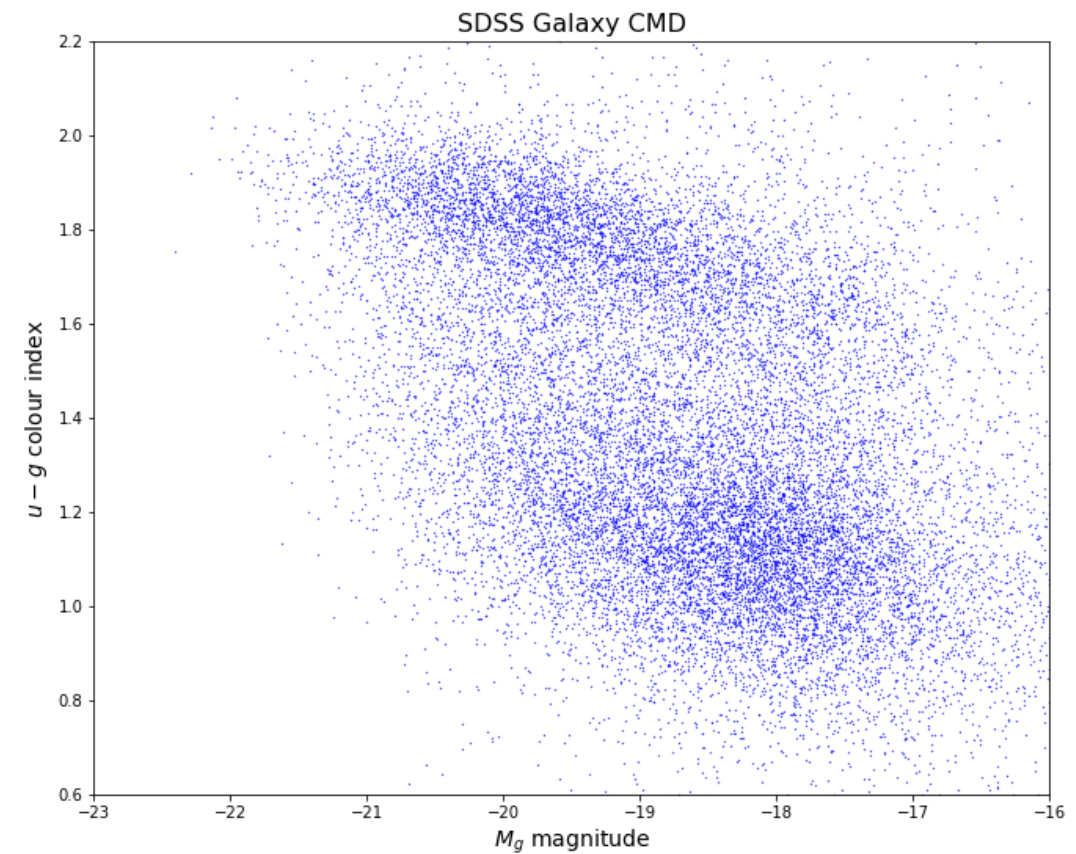
\includegraphics[width=\columnwidth]{images/CMDs/galaxyCMD.PNG}
    \caption{Galaxy colour-magnitude diagram: $u-g$ colour index versus $M_g$ magnitude. The bimodality of the distribution is discussed in the text.}
    \label{fig:CMD1}
\end{figure}

\subsection{Structure}
The content of the paper is organised as follows: Section \ref{sec:sample} describes the conditions required for PSB sample and the corresponding control galaxies. Data analysis methods are discussed in Section \ref{sec:analysis}. Finally, a summary of the research and the conclusions drawn from this work, along with recommendations for further study are presented in Section \ref{sec:discussion}.
